\let\negthickspace\undefined
\documentclass[journal,12pt,twocolumn]{IEEEtran}
\usepackage{cite}
\usepackage{amsmath,amssymb,amsfonts,amsthm}
\usepackage{algorithmic}
\usepackage{graphicx}
\usepackage{textcomp}
\usepackage{xcolor}
\usepackage{txfonts}
\usepackage{listings}
\usepackage{enumitem}
\usepackage{mathtools}
\usepackage{gensymb}
\usepackage{comment}
\usepackage[breaklinks=true]{hyperref}
\usepackage{tkz-euclide} 
\usepackage{listings}
\usepackage{gvv}                                        
\def\inputGnumericTable{}                                 
\usepackage[latin1]{inputenc}                                
\usepackage{color}                                            
\usepackage{array}                                            
\usepackage{longtable}                                       
\usepackage{calc}                                             
\usepackage{multirow}                                         
\usepackage{hhline}                                           
\usepackage{ifthen}                                           
\usepackage{lscape}
\setlength{\arrayrulewidth}{0.5mm}
\setlength{\tabcolsep}{18pt}
\renewcommand{\arraystretch}{1.5}
\newtheorem{theorem}{Theorem}[section]
\newtheorem{problem}{Problem}
\newtheorem{proposition}{Proposition}[section]
\newtheorem{lemma}{Lemma}[section]
\newtheorem{corollary}[theorem]{Corollary}
\newtheorem{example}{Example}[section]
\newtheorem{definition}[problem]{Definition}
\newcommand{\BEQA}{\begin{eqnarray}}
\newcommand{\EEQA}{\end{eqnarray}}
\newcommand{\define}{\stackrel{\triangle}{=}}
\theoremstyle{remark}
\newtheorem{rem}{Remark}
\begin{document}
\title{Progressions (7) 11.9.5}
\author{EE23BTECH11051-Rajnil Malviya}
\date{January 2024}
\maketitle
\subsection*{\textit{Question :-}}
If a function Satisfying f\brak {x+y} = f\brak{x} f\brak{y} for all $x,y \in {N}$ such that f\brak {1} =3 and $\sum_{x=1}^{n} f\brak{x} = 120$ , find the value of n .\\
\textit{Solution:- }
  $x=1$ and $y=1$ , we get
\begin{align}
    f\brak2&=f\brak{1+1} ={f\brak1} f\brak 1\\
      f\brak3&=f\brak{2+1} ={f\brak2} f\brak 1\\
        f\brak4&=f\brak{3+1} ={f\brak3} f\brak 1
        \end{align}
        Using induction , we get ;
       \begin{align}
           f\brak x&=f\brak{(x-1)+1} ={f\brak{x-1}} f\brak 1\\
           \implies f\brak{x }&=[f\brak 1]^x
       \end{align}
       


so it is a GP with common ratio $r=3 ;$


\begin{table}[h!]
        \begin{tabular}{ | m{1.0cm} | m{3cm} |m{1cm} |} 
  \hline
 Symbol &Description& Value \\ 
 \hline
$x(0)$&first term& 3  \\
\hline
$r$&common ratio & 3  \\
\hline
$y\brak n$& sum of all n terms&120 \\
\hline
$x(n)$&${n+1}^{th}$ term& $ x \brak 0r^{n}$\\
\hline
\end{tabular}\\
\caption{}
\label{Table:1}
    
    \end{table}

Applying z-transformation on x\brak n ;
\begin{align}
\implies X(z) &=\frac{3}{1-3z^{-1}} \quad \abs{z} > \abs{3}\\
Y \brak z &= X\brak zU\brak z\\
\implies Y(z)&=\brak{\frac{3}{1-3 z^{-1}}}\brak{\frac{1}{1- z^{-1}}}  \quad \abs{z} > \abs{r}
\end{align}
Using contour integration  ;
\begin{align}
   y(n) &=\frac{1}{2\pi j}\oint_{C}{\frac{3}{\brak{1-3 z^{-1}}\brak{1- z^{-1}}}}  \;dz 
\end{align}
We can observe two non repeated poles $z=3$ and $z=1$
\begin{align}
    R_1&=\lim\limits_{z\to 3} \brak{z-3} \frac{3 z^{n+1}}{\brak{z-3}\brak{z-1}}\\
  &=\frac{3^{n+2}}{2}\\
   R_2&=\lim\limits_{z\to 1} \brak{z-1} \frac{3 z^{n+1}}{\brak{z-3}\brak{z-1}}\\
  &=\frac{-3}{2}\\
  y\brak n&= R_1+R_2\\
   &=\frac{3^{n+2}}{2}+\frac{-3}{2} \\
  \implies 120&=\frac{3^{n+2}-3}{2} \\
   \implies n&=3
\end{align}
Ans . $n$ take values from $n=0$ to  $n=3$, so there are total four terms .
\newpage
\begin{figure}
   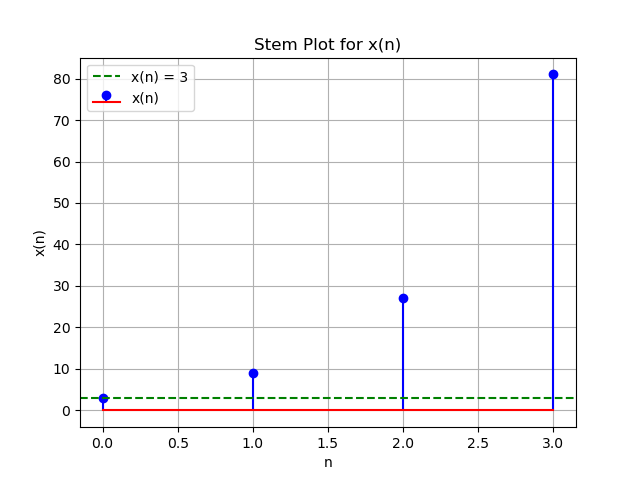
\includegraphics[width=1\linewidth]{figs/i1.png}
\end{figure}
\begin{figure}
   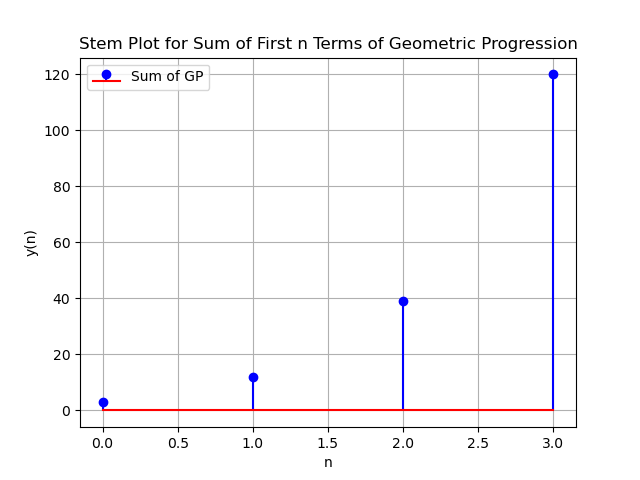
\includegraphics[width=1\linewidth]{figs/i2.png}
\end{figure}
\end{document}
